\section{Monitor Object}


The Monitor Object design pattern synchronizes concurrent method
execution to ensure that only one method at a time runs within an
object. It also allows an object’s methods to cooperatively schedule
their execution sequences.

\subsection*{Problem}


Mehrere Threads greifen gleichzeitig auf Methoden desselben Objektes zu. Die Methoden ändern Felder des Objektes, was somit dessen Zustand ändert. Um dies zu gewährleisten, müssen folgende Probleme berücksichtig werden:


\begin{enumerate}
	\item Es sollten nur Interfaceaufrufe, welche die Synchronisation definieren, auf dem Objekt aufgerufen werden. Zur gleichen Zeit sollte auf dem Objekt immer nur 1 Methode ausgeführt werden.
	\item Da Lowlevel Synchronisation komplex ist, soll sich das Objekt selbst um selbige kümmern.
	\item Um Deadlocks vorzubeugen/zu vermeiden, müssen blockierende Threads den Lock selbstständig freigeben.
	\item Bei der freiwilligen Abgabe muss das Objekt jedoch in einem stabilen Zustand sein.
\end{enumerate}

\subsection*{Lösung}


Jedes Objekt, welches vor parallelem Zugriff geschützt werden sollte, muss einen Monitor Lock implementieren. Die Methoden, welche als synchronized deklariert sind, teilen sich einen gemeinsamen Montitor Lock. Wird dieser Monitor Lock von einer Methode beansprucht, können andere synchronized Methoden nicht zur Ausführung kommen. Die Kommunikation zwischen den Threads geschieht dann über die sogenannten Monitor Conditions (wait(), notify(), notifyAll(),..), worüber die Methoden die Ausführung selbst stoppen und wiederaufnehmen können.


\begin{figure}[H]
	\centering
	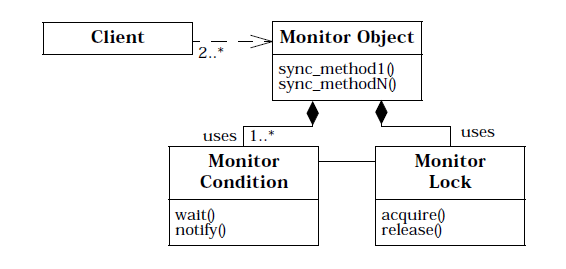
\includegraphics[width=\textwidth]{content/posa2/monitor-object/images/UML.png}
	\caption{UML}
\end{figure}


\begin{figure}[H]
	\centering
	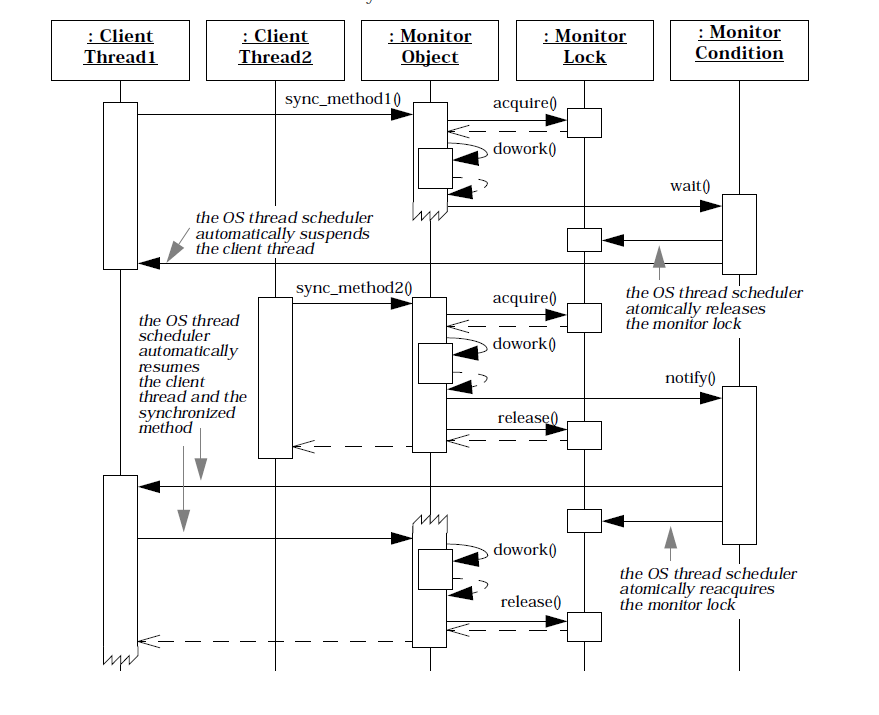
\includegraphics[width=\textwidth]{content/posa2/monitor-object/images/SSD.png}
	\caption{SSD}
\end{figure}


\subsection*{Implementation}

\begin{enumerate}
	\item Monitor Object Interface definieren
	\item Von aussen zugängliche Methode definieren
	\item Monitor Lock definieren (nur 1 Methode pro Objekt)
	\item Monitor Condition definieren (Kommunikation zwischen Threads)
\end{enumerate}


\subsection*{Varianten}

\begin{itemize}
	\item Timed Synchronisation Method Invocations
	\begin{itemize}
		\item Maximale Wartezeit kann definiert werden
	\end{itemize}
	\item Strategized Locking
	\begin{itemize}
		\item Mehrere Monitor Locks/Condition definieren
	\end{itemize}
\end{itemize}

\subsection*{Vorteile}


\begin{itemize}
	\item Parallelprogrammierung (Kontrolle) wird vereinfacht
	\item Vereinfachung der Planung der Methodenausführungen. Mit Hilfe der Monitor Conditions (wait()..)
\end{itemize}

\subsection*{Nachteile}


\begin{itemize}
	\item Skalierbarkeit wird beeinträchtigt, wenn mehrere Threads um den Monitor Lock kämpfen
	\item Monitor Object Synchronisation ist oft eng an die Methodenfunktionalität gebunden
	\item Vererbung von der Basisklasse ist nicht immer einfach, falls ein anderer Synchronisationsmechanismus zum Einsatz kommt
	\item Nested monitor lockout: Methoden können sich gegenseitig ausschliessen (durch Verschachtelung von Monitor Locks)
\end{itemize}

\subsection*{Known Uses}


\begin{itemize}
	\item Dijkstra and Hoare-style Monitors
	\item Java Objects
	\item ACE Gateway
	\item Fast food restaurant
\end{itemize}

\subsection*{Prüfungsfragen}


\begin{itemize}
	\item Wie kann es bei Monitor-Objects zu Deadlocks kommen? Wie viele Monitor-Objects müssen dabei mindestens involviert sein?
\end{itemize}

